%%===============================================================
%%===============================================================
\chapter{Setting up the development environment for OpenFCST}
%%===============================================================
%%===============================================================
%% Author: Phil Wardlaw and Marc Secanell
%%===============================================================
%%===============================================================

In the following sections we describe how to create an OpenFCST branch where you can develop your own code and commit the changes to the OpenFCST team. Also, we show how to setup KDevelop, the program we recommend for compiling and modifying code in OpenFCST.

%%===============================================================
\section{Getting the \texttt{development} version of OpenFCST}

The development version of OpenFCST is hosted on a private repository on BitBucket. In order to access the \texttt{development} branch of OpenFCST, please contact the developers. You can also develop code from the GitHub version of the code and then submit your changes to the OpenFCST team. We will then merge the changes into the code for the next release.

If you want to modify OpenFCST, you will need to first clone the development version of OpenFCST, and then create your own branch of the code. Afterwards you can then modify, test, and commit this branch. Once your branch has been tested and validated, you can issue a Pull Request. Then, several senior OpenFCST developers will look at the code, suggest changes, and finally merge the code into the stable development version of OpenFCST. The stable development version of OpenFCST is then used to create new releases.

%%=======
\subsubsection{Creating a new branch}

Committing changes to the development branch is not allowed. You will need to create a pull request of your branch. Every user can create their own branch of OpenFCST. The recommended convention for branch usage is that each user creates their own branch for each issue in OpenFCST they would like to address. The naming convention is: \texttt{username/issue\_name}. For example, if Secanell wants to create an issue to fix a bug on postprocessing, the branch would be named \texttt{secanell/postprocessing}.
 
To create a branch, users can either create it on their own machine and then push it to BitBucket or create the branch directly on BitBucket. If the branch is created on BitBucket, then, in order to checkout the branch to the appropriate machine, the user needs to issue the following command:
\begin{lstlisting}
  git branch branch_name origin/branch_name  
  git checkout branch_name
\end{lstlisting}  
Both steps can be performed simultaneously with
\begin{lstlisting}
git checkout -b username/issue\_name origin/username/issue\_name}
\end{lstlisting}  
 
If the branch is created on the local repository first using \texttt{git checkout -b branch\_name}, then you can commit it to BitBucket, i.e. remote server, using \texttt{git push -u origin branch\_name}.
The \texttt{-u} flag means that from now on your branch \texttt{branch\_name} will track the branch on BitBucket.

%%=======
\subsubsection{Adding, changing, staging, committing and pushing}
 
Once the branch is created, users can work on that branch for as long as needed. Users can make changes and commit the changes to their local repository using:
\begin{lstlisting}
  git add file_name
  git commit -m "message about commit"
\end{lstlisting} 
Please DO NOT use \texttt{git add *} or \texttt{git add -u} as you then have little control over what you are staging to be  committed. Using \texttt{git status} you can see which files have changed so that you can add them
as appropriate.
 
To commit to BitBucket, you can use:
\begin{lstlisting}
  git push origin branch_name
\end{lstlisting} 

%%=======
\subsubsection{Request for branch to be merged into development}

Once you have finished fixing the issue you created the branch for, you need to follow these three steps:
\begin{enumerate}
 \item Update your origin information using: \texttt{git remote update} (this will update all your local information regarding the branches on BitBucket).
 \item Merge your branch with the latest version of development using: \texttt{git merge origin/development}. This is VERY important. The administration will not accept any pull requests that 
   have not been fast-forwarded to the \texttt{origin/development branch}.
 \item Issue a pull request in BitBucket
\end{enumerate}

 
There are three main branches  
\begin{itemize}
 \item Master branch: Stable version of OpenFCST (no pull requests will be accepted to this branch).
 \item Development branch: The most up-to-date version of OpenFCST, personal branches should be started from this branch and all pull requests should be submitted to this branch.
 \item Release branch: Branch containing the latest release of OpenFCST.
\end{itemize}

%==================
\subsubsection{Workflow for new development}

If you want to develop new code, please follow these steps: 
\begin{itemize}
 \item Clone the repository using:\\
  \texttt{git clone https://your\_username@bitbucket.org/ESDLab/openfcst.git}
 \item Create a new branch related to the new component/issue you would like to work on using: \texttt{git checkout -b name\_branch}. Note: The command above will create a branch named \texttt{name\_branch} and will checkout that branch so you are ready to work.
 \item Once you are done with the development, ask for a pull request to merge your branch to the development branch.
\end{itemize}
Note: Merges to Master will be rejected without review.

A reminder: when developing code, please work on Debug mode (the current version gives an error once the program finishes in debug mode, please ignore for now as we will be working on fixing this) and test on Debug and Release mode before issuing a pull request. We are aware that running tests in Debug is more time consuming, but the issues that we have in debug mode have occurred precisely because we did not test on that mode.


%%===============================================================
\section{Setting up OpenFCST under KDevelop} \label{setting_up_fcst}
%%===============================================================

If you are going to be developing new routines for OpenFCST, we recommend that you use either KDevelop or Eclipse to modify, compile, and debug new code. In order to setup a KDevelop project with OpenFCST, follow the steps below:
\begin{itemize}
 \item Compile OpenFCST using the provided script, i.e. \texttt{openFCST\_install}. This will configure all the folders you will be using during configuration  of KDevelop. This step is not required, however, it is recommended and the steps below assume OpenFCST has been installed and that the Build and Install directories already exist on your computer.
 \item Go to Project $>$ Open/Import Project... Go to the OpenFCST folder, enter the \texttt{src} folder and then, select the \texttt{CMakeLists.txt} file in \texttt{openfcst/src} (see Figure \ref{fig:setup_KDevelop}). In the next window, enter the name of the project, e.g. OpenFCST, and select \texttt{CMake Project Manager}. At this point, the project should either appear or prompt another window asking for the Build folder. If the latter is the case, point KDevelop to the Build folder in the main folder of OpenFCST. Then, the project import is complete and the project menu will appear on the left hand side.
 \item If you want to modify the compilation parameters in the project, you can do that by right clicking on the project name and selecting \texttt{Open Configuration...}. The menu in Figure \ref{fig:setup_KDevelop_options} would appear. You should not need to modify many parameters, however several parameters are handy. The variable OPEN\_FCST\_BUILD\_TYPE allows you to compile the code in Debug or Release mode. The former is used during code development as it provides a lot more information about errors, the latter is best for simulations as the code can be several times faster. Another useful parameter is OPEN\_FCST\_DIMENSIONS. If set to 2, it will only compile a 2D version of OpenFCST. If you compile with 3, it will compile a 3D version. If you compile with 1, it will compile both 2D and 3D versions. Finally, on the left menu if you click on Make, the parameter \texttt{Number of simultaneous jobs} sets up the compilation for using as many threads as specified. 
\end{itemize}

\begin{figure}[btp]
\begin{center} 
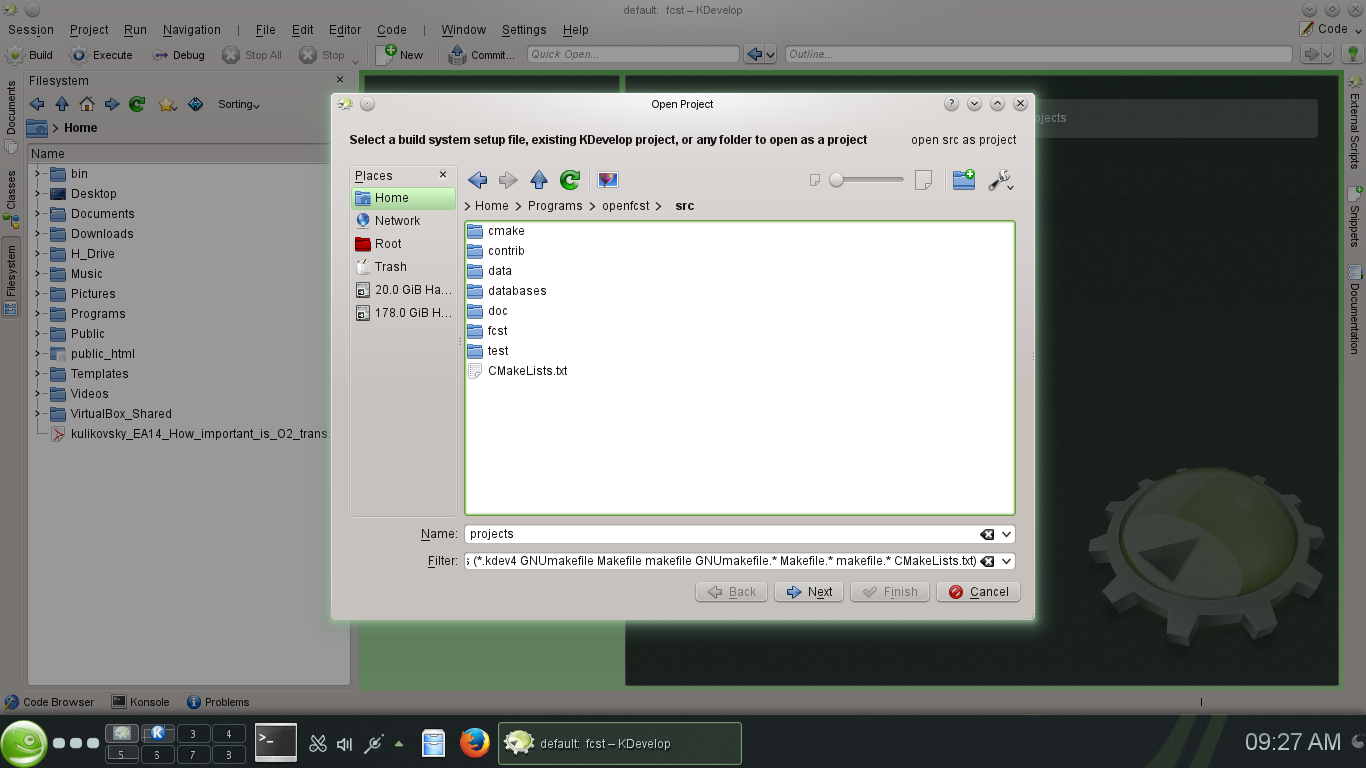
\includegraphics[width=\textwidth]{./figures/kdevelop_1.png}
\caption{Initial window in KDevelop to import a CMake project.}
\label{fig:setup_KDevelop}
\end{center}
\end{figure}

\begin{figure}[btp]
\begin{center} 
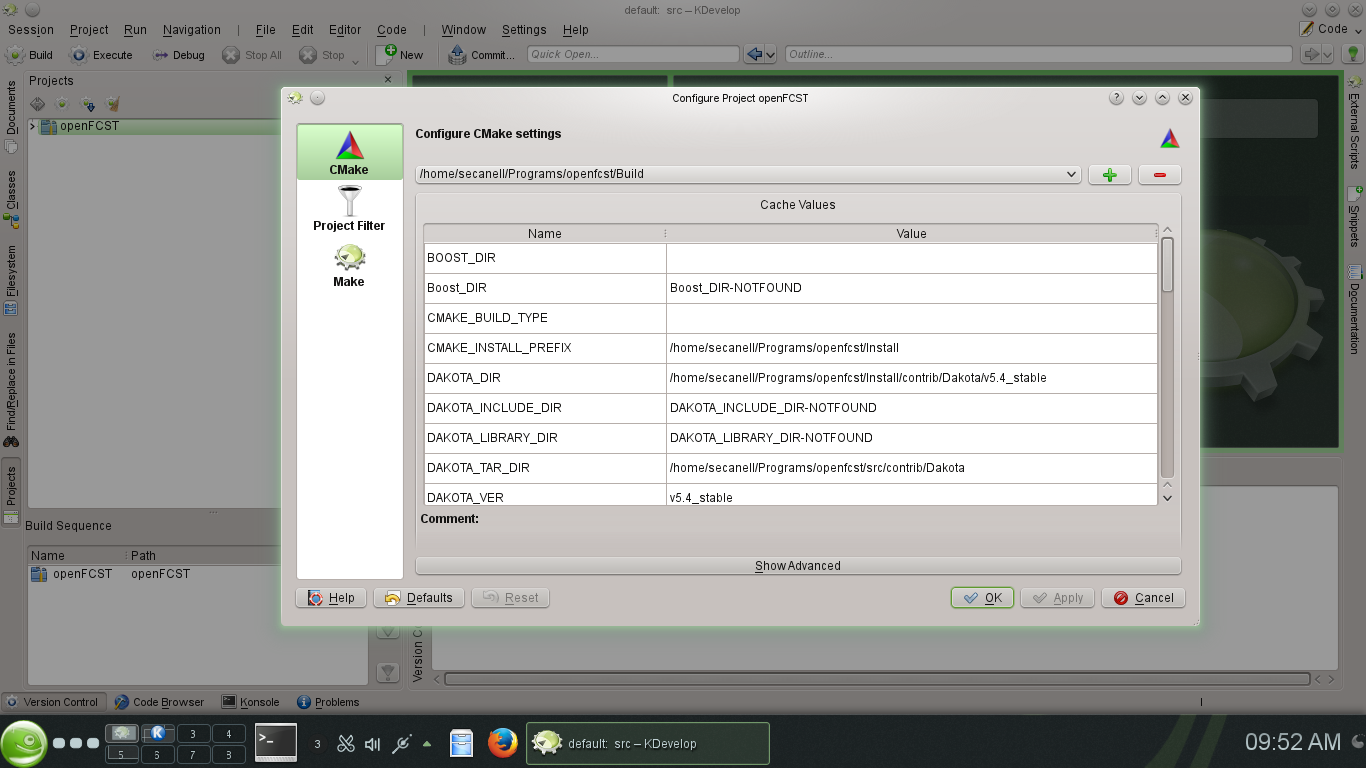
\includegraphics[width=\textwidth]{./figures/kdevelop_2.png}
\caption{Configuring your CMake project in KDevelop.}
\label{fig:setup_KDevelop_options}
\end{center}
\end{figure}

Next, we will setup the environment to run and debug OpenFCST within KDevelop by following the steps below:
\begin{itemize}
 \item Go to \texttt{Run $>$ Configure Launches... }. The window in Figure \ref{fig:example_KDevelop} will open.
 \item Select either Global or your project option (we recommend your project).
 \item Press the '+' button on the top of the window. Once you press this botton, a new option will open under either Global or OpenFCST. 
 \item Select \texttt{New Native Application Configuration}, then on the right of the window, under Executables, enter the OpenFCST binary file, i.e. \texttt{OpenFCST\_directory/Install/bin/fuel\_cell-2d.bin}. Under Behaviour, in Working Directory enter the data folder from which you would like to run the code. In Arguments, enter the main parameter file, see Figure \ref{fig:example_KDevelop}.
 \item Your code is set! Click OK on the window. Now, you can run the code with the \texttt{Execute} and \texttt{Debug...} buttons on the menu. If you have more than one \texttt{New Native Application Configuration} configured, rename them by clicking on the same. Then, you can switch between application configurations using \texttt{Run $>$ Current Launch Configuration}
\end{itemize}
 
\begin{figure}[btp]
\begin{center} 
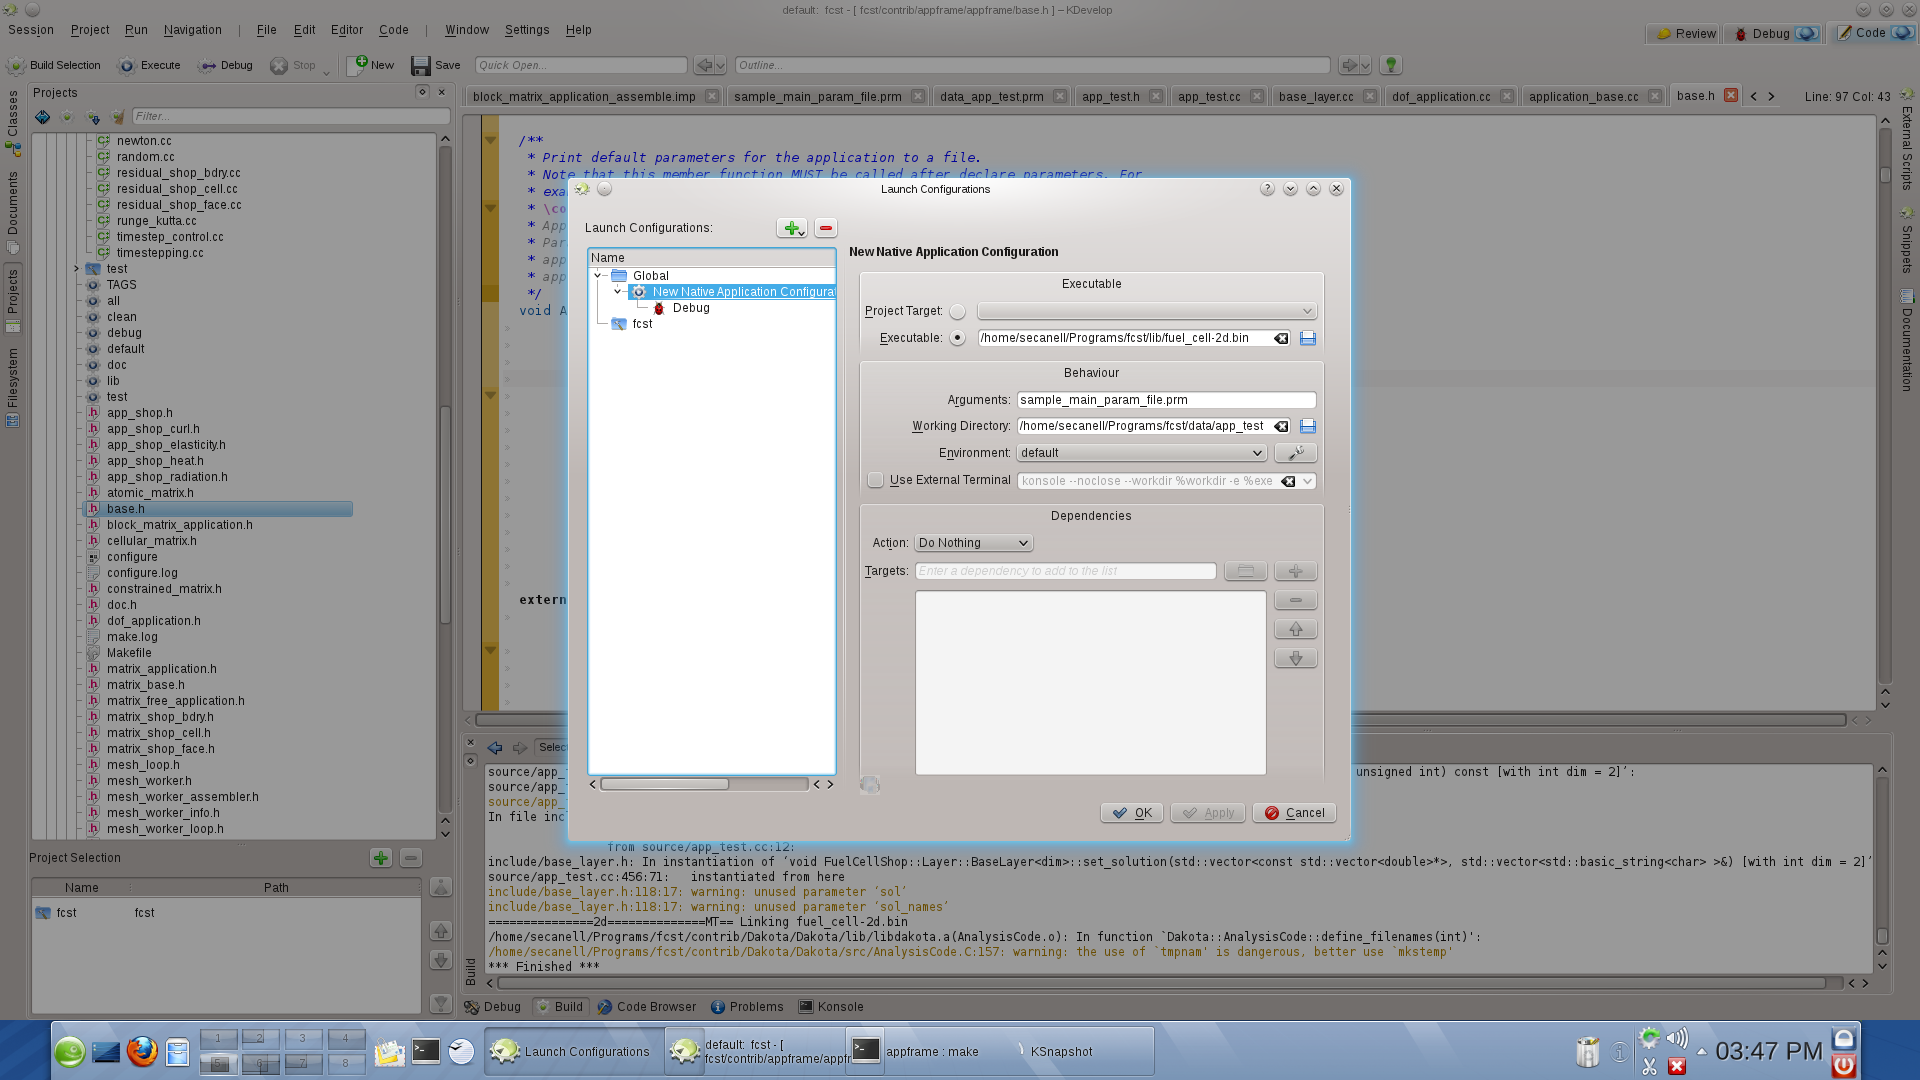
\includegraphics[width=\textwidth]{./figures/LaunchConfigurations.png}
\caption{Configuring Launches in KDevelop.}
\label{fig:example_KDevelop}
\end{center}
\end{figure}

\subsection{Formatting OpenFCST files}

All files should start with the following information:

\begin{lstlisting}
// ----------------------------------------------------------------------------
//
// FCST: Fuel Cell Simulation Toolbox
//
// Copyright (C) 2009-20XX by Energy Systems Design Laboratory, University of Alberta
//
// This software is distributed under the MIT License
// For more information, see the README file in /doc/LICENSE
//
// - Class: class_name
// - Description: short description of class
// - Developers: name_developers, affiliation
// - Id: $Id$
//
// ----------------------------------------------------------------------------
\end{lstlisting}
 
In order to keep the formatting of all files consistent, it is recommended to use the space style for code readability. In KDevelop, set your formatting options:
\begin{itemize}
\item In the main menu, go to Setting $>$ Configure Editor.
\item In the 'Editing' section, select the Indentation tab.
\item Set 'Indent Using' to \textit{Spaces}, and set the spacing to \textbf{4 characters}. 
\end{itemize}
%%===============================================================
%%==============================================================